\begin{figure}
  \centering
  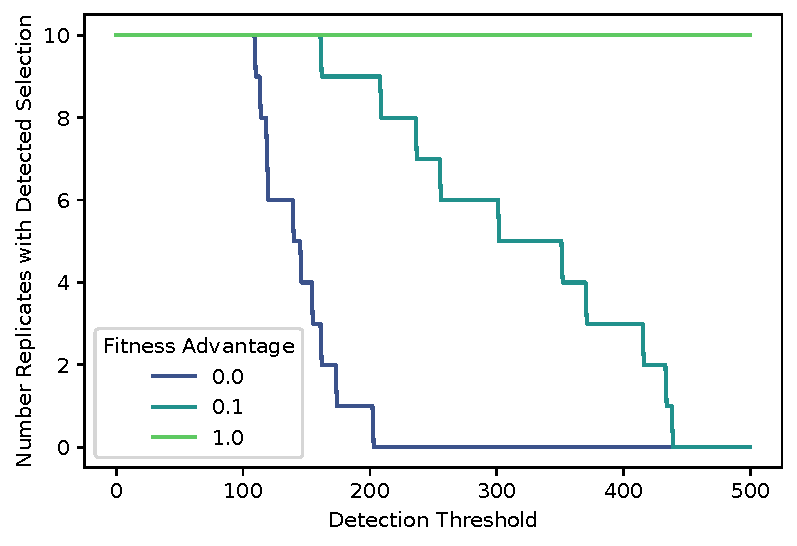
\includegraphics[width=0.8\textwidth]{notebooks/notebooks/teeplots/hue=fitness-advantage+viz=lineplot-detection+x=threshold+y=replicate-count+ext=}
  \caption{
    Gene selection detection rates across detection thresholds for each fitness advantage level among 10 replicates.
    Fitness advantage 0.0 inferred no selective benefit, so all selection detections on this treatment are false positives.
    Fitness advantage 0.1 experienced relatively weak selection and fitness advantage 1.0 experienced strong selection.
    Detection threshold 200 distinguishes treatment 0.0 and 0.1 with one false positive and one false negative.
    Fitness advantage 1.0 has all replicates detected across all shown threshold values.
    Selection is detected for a replicate if any 16-generation rolling sum of gene prevalence annotation bit count (Section \ref{sec:dist-gene-prevalence-est}) exceeds the threshold.
  }
  \label{fig:selection-sensitivity-specificity}
\end{figure}
